% This file was created by tikzplotlib v0.9.8.
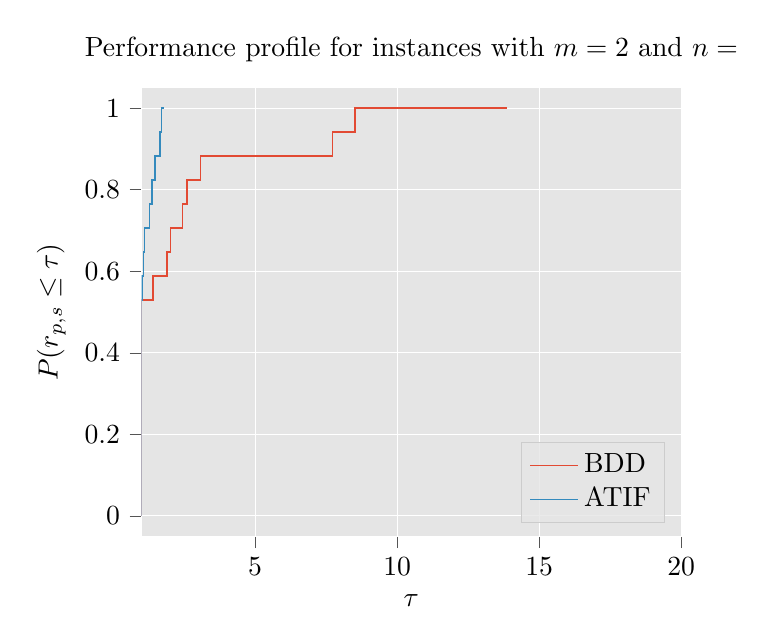
\begin{tikzpicture}

\definecolor{color0}{rgb}{0.886274509803922,0.290196078431373,0.2}
\definecolor{color1}{rgb}{0.203921568627451,0.541176470588235,0.741176470588235}

\begin{axis}[
axis background/.style={fill=white!89.8039215686275!black},
axis line style={white},
legend cell align={left},
legend style={
  fill opacity=0.8,
  draw opacity=1,
  text opacity=1,
  at={(0.97,0.03)},
  anchor=south east,
  draw=white!80!black,
  fill=white!89.8039215686275!black
},
tick align=outside,
tick pos=left,
title={Performance profile for instances with \(\displaystyle m = 2\) and \(\displaystyle n = \)},
x grid style={white},
xlabel={\(\displaystyle \tau\)},
xmajorgrids,
xmin=1, xmax=20,
xtick style={color=white!33.3333333333333!black},
y grid style={white},
ylabel={\(\displaystyle P(r_{p,s} \leq \tau)\)},
ymajorgrids,
ymin=-0.05, ymax=1.05,
ytick style={color=white!33.3333333333333!black}
]
\addplot [semithick, color0, const plot mark right]
table {%
1 0
1 0.0588235294117647
1 0.117647058823529
1 0.176470588235294
1 0.235294117647059
1 0.294117647058824
1 0.352941176470588
1 0.411764705882353
1 0.470588235294118
1.39918977707006 0.529411764705882
1.88864439823009 0.588235294117647
2.02073988625592 0.647058823529412
2.43812394904459 0.705882352941177
2.60807914285714 0.764705882352941
3.07839526027397 0.823529411764706
7.72928091525424 0.882352941176471
8.50831248275862 0.941176470588235
13.8621281460674 1
};
\addlegendentry{BDD}
\addplot [semithick, color1, const plot mark right]
table {%
1 0
1 0.0588235294117647
1 0.117647058823529
1 0.176470588235294
1 0.235294117647059
1 0.294117647058824
1 0.352941176470588
1 0.411764705882353
1 0.470588235294118
1.02277826465031 0.529411764705882
1.07521908682651 0.588235294117647
1.10580222833303 0.647058823529412
1.2809226080609 0.705882352941177
1.37905436277936 0.764705882352941
1.46391509722209 0.823529411764706
1.6483276327126 0.882352941176471
1.70716257842723 0.941176470588235
1.78252211600654 1
};
\addlegendentry{ATIF}
\end{axis}

\end{tikzpicture}
